\documentclass[1p]{elsarticle_modified}
%\bibliographystyle{elsarticle-num}

%\usepackage[colorlinks]{hyperref}
%\usepackage{abbrmath_seonhwa} %\Abb, \Ascr, \Acal ,\Abf, \Afrak
\usepackage{amsfonts}
\usepackage{amssymb}
\usepackage{amsmath}
\usepackage{amsthm}
\usepackage{scalefnt}
\usepackage{amsbsy}
\usepackage{kotex}
\usepackage{caption}
\usepackage{subfig}
\usepackage{color}
\usepackage{graphicx}
\usepackage{xcolor} %% white, black, red, green, blue, cyan, magenta, yellow
\usepackage{float}
\usepackage{setspace}
\usepackage{hyperref}

\usepackage{tikz}
\usetikzlibrary{arrows}

\usepackage{multirow}
\usepackage{array} % fixed length table
\usepackage{hhline}

%%%%%%%%%%%%%%%%%%%%%
\makeatletter
\renewcommand*\env@matrix[1][\arraystretch]{%
	\edef\arraystretch{#1}%
	\hskip -\arraycolsep
	\let\@ifnextchar\new@ifnextchar
	\array{*\c@MaxMatrixCols c}}
\makeatother %https://tex.stackexchange.com/questions/14071/how-can-i-increase-the-line-spacing-in-a-matrix
%%%%%%%%%%%%%%%

\usepackage[normalem]{ulem}

\newcommand{\msout}[1]{\ifmmode\text{\sout{\ensuremath{#1}}}\else\sout{#1}\fi}
%SOURCE: \msout is \stkout macro in https://tex.stackexchange.com/questions/20609/strikeout-in-math-mode

\newcommand{\cancel}[1]{
	\ifmmode
	{\color{red}\msout{#1}}
	\else
	{\color{red}\sout{#1}}
	\fi
}

\newcommand{\add}[1]{
	{\color{blue}\uwave{#1}}
}

\newcommand{\replace}[2]{
	\ifmmode
	{\color{red}\msout{#1}}{\color{blue}\uwave{#2}}
	\else
	{\color{red}\sout{#1}}{\color{blue}\uwave{#2}}
	\fi
}

\newcommand{\Sol}{\mathcal{S}} %segment
\newcommand{\D}{D} %diagram
\newcommand{\A}{\mathcal{A}} %arc


%%%%%%%%%%%%%%%%%%%%%%%%%%%%%5 test

\def\sl{\operatorname{\textup{SL}}(2,\Cbb)}
\def\psl{\operatorname{\textup{PSL}}(2,\Cbb)}
\def\quan{\mkern 1mu \triangleright \mkern 1mu}

\theoremstyle{definition}
\newtheorem{thm}{Theorem}[section]
\newtheorem{prop}[thm]{Proposition}
\newtheorem{lem}[thm]{Lemma}
\newtheorem{ques}[thm]{Question}
\newtheorem{cor}[thm]{Corollary}
\newtheorem{defn}[thm]{Definition}
\newtheorem{exam}[thm]{Example}
\newtheorem{rmk}[thm]{Remark}
\newtheorem{alg}[thm]{Algorithm}

\newcommand{\I}{\sqrt{-1}}
\begin{document}

%\begin{frontmatter}
%
%\title{Boundary parabolic representations of knots up to 8 crossings}
%
%%% Group authors per affiliation:
%\author{Yunhi Cho} 
%\address{Department of Mathematics, University of Seoul, Seoul, Korea}
%\ead{yhcho@uos.ac.kr}
%
%
%\author{Seonhwa Kim} %\fnref{s_kim}}
%\address{Center for Geometry and Physics, Institute for Basic Science, Pohang, 37673, Korea}
%\ead{ryeona17@ibs.re.kr}
%
%\author{Hyuk Kim}
%\address{Department of Mathematical Sciences, Seoul National University, Seoul 08826, Korea}
%\ead{hyukkim@snu.ac.kr}
%
%\author{Seokbeom Yoon}
%\address{Department of Mathematical Sciences, Seoul National University, Seoul, 08826,  Korea}
%\ead{sbyoon15@snu.ac.kr}
%
%\begin{abstract}
%We find all boundary parabolic representation of knots up to 8 crossings.
%
%\end{abstract}
%\begin{keyword}
%    \MSC[2010] 57M25 
%\end{keyword}
%
%\end{frontmatter}

%\linenumbers
%\tableofcontents
%
\newcommand\colored[1]{\textcolor{white}{\rule[-0.35ex]{0.8em}{1.4ex}}\kern-0.8em\color{red} #1}%
%\newcommand\colored[1]{\textcolor{white}{ #1}\kern-2.17ex	\textcolor{white}{ #1}\kern-1.81ex	\textcolor{white}{ #1}\kern-2.15ex\color{red}#1	}

{\Large $\underline{12a_{0122}~(K12a_{0122})}$}

\setlength{\tabcolsep}{10pt}
\renewcommand{\arraystretch}{1.6}
\vspace{1cm}\begin{tabular}{m{100pt}>{\centering\arraybackslash}m{274pt}}
\multirow{5}{120pt}{
	\centering
	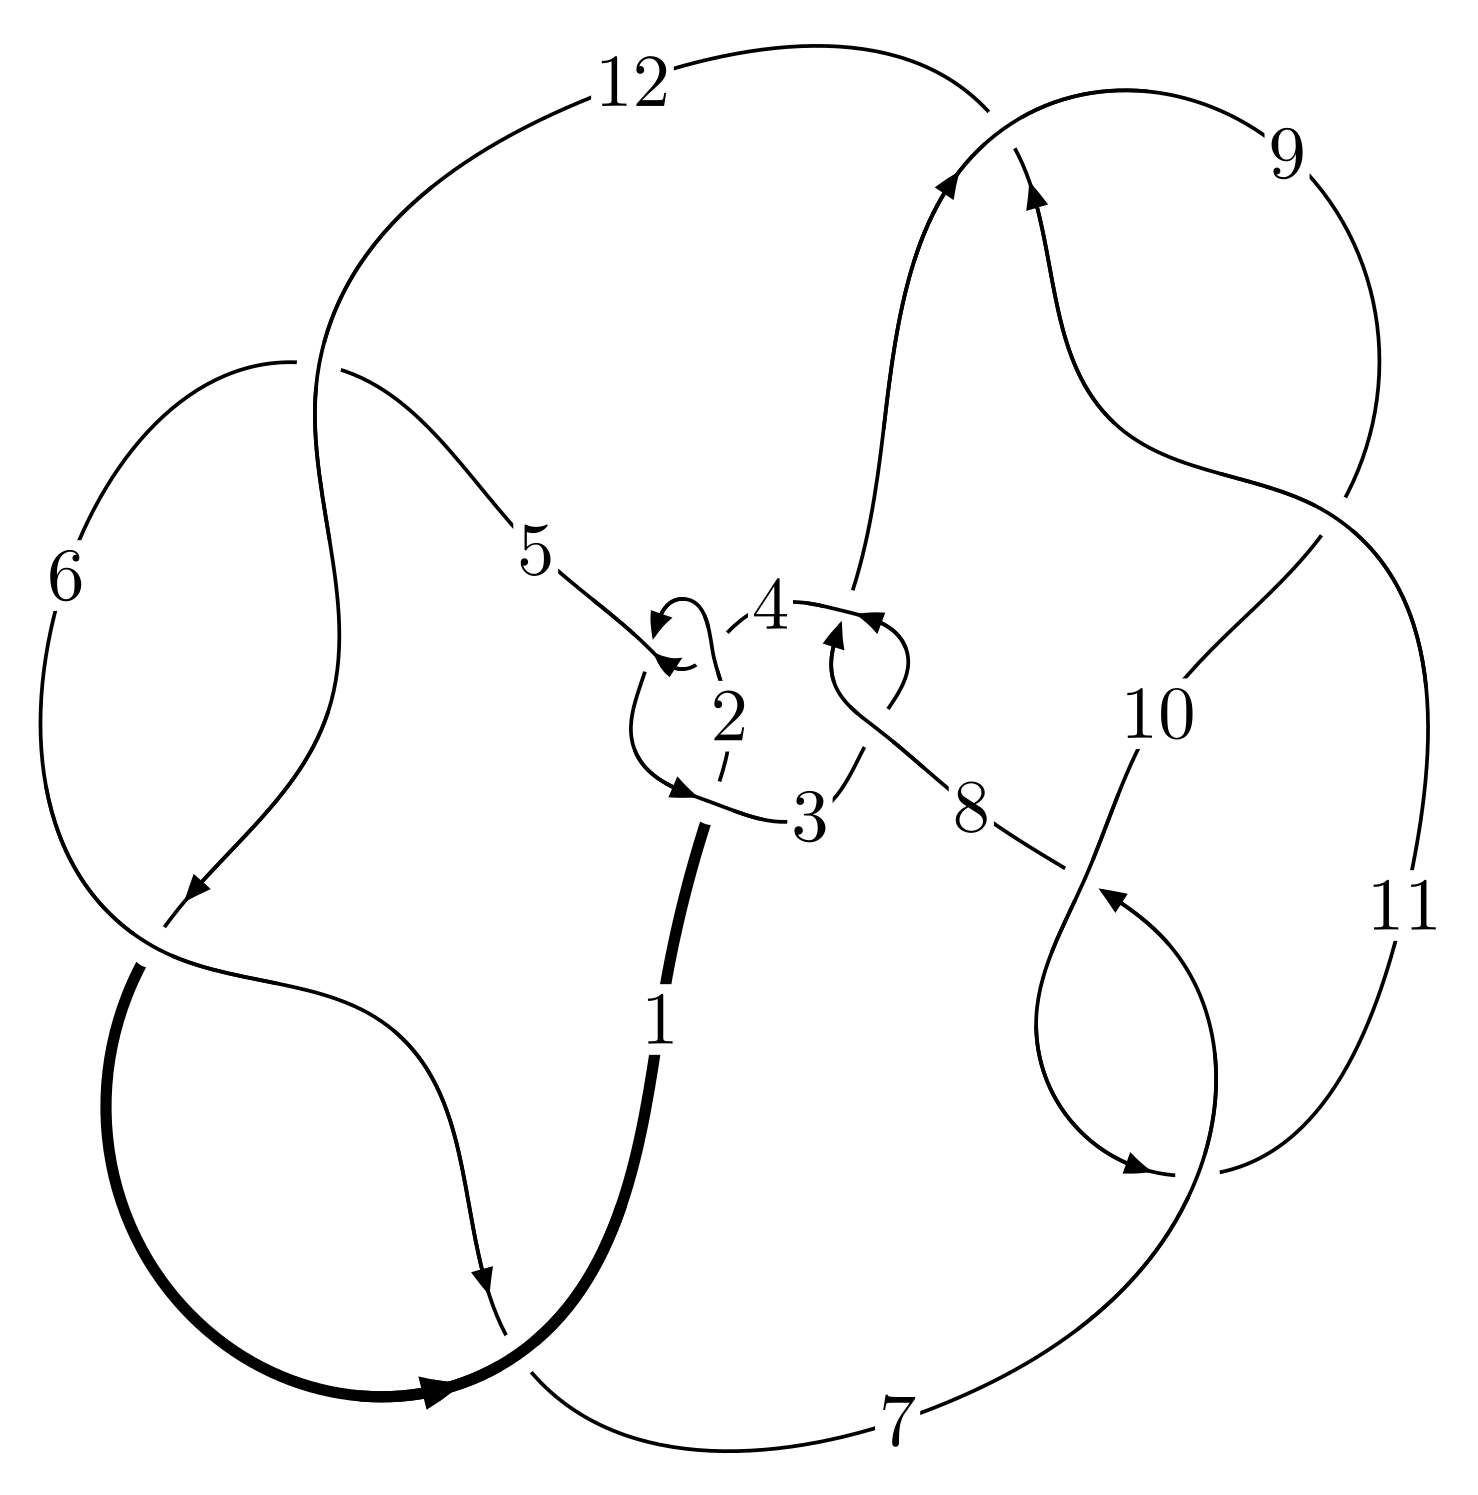
\includegraphics[width=112pt]{../../../GIT/diagram.site/Diagrams/png/923_12a_0122.png}\\
\ \ \ A knot diagram\footnotemark}&
\allowdisplaybreaks
\textbf{Linearized knot diagam} \\
\cline{2-2}
 &
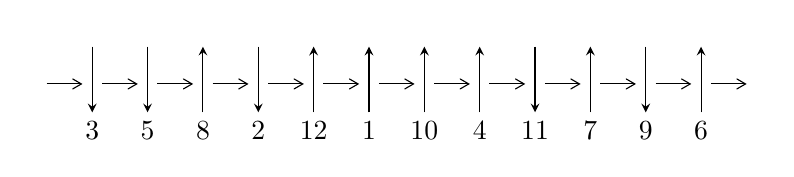
\begin{tikzpicture}[x=20pt, y=17pt]
	% nodes
	\node (C0) at (0, 0) {};
	\node (C1) at (1, 0) {};
	\node (C1U) at (1, +1) {};
	\node (C1D) at (1, -1) {3};

	\node (C2) at (2, 0) {};
	\node (C2U) at (2, +1) {};
	\node (C2D) at (2, -1) {5};

	\node (C3) at (3, 0) {};
	\node (C3U) at (3, +1) {};
	\node (C3D) at (3, -1) {8};

	\node (C4) at (4, 0) {};
	\node (C4U) at (4, +1) {};
	\node (C4D) at (4, -1) {2};

	\node (C5) at (5, 0) {};
	\node (C5U) at (5, +1) {};
	\node (C5D) at (5, -1) {12};

	\node (C6) at (6, 0) {};
	\node (C6U) at (6, +1) {};
	\node (C6D) at (6, -1) {1};

	\node (C7) at (7, 0) {};
	\node (C7U) at (7, +1) {};
	\node (C7D) at (7, -1) {10};

	\node (C8) at (8, 0) {};
	\node (C8U) at (8, +1) {};
	\node (C8D) at (8, -1) {4};

	\node (C9) at (9, 0) {};
	\node (C9U) at (9, +1) {};
	\node (C9D) at (9, -1) {11};

	\node (C10) at (10, 0) {};
	\node (C10U) at (10, +1) {};
	\node (C10D) at (10, -1) {7};

	\node (C11) at (11, 0) {};
	\node (C11U) at (11, +1) {};
	\node (C11D) at (11, -1) {9};

	\node (C12) at (12, 0) {};
	\node (C12U) at (12, +1) {};
	\node (C12D) at (12, -1) {6};
	\node (C13) at (13, 0) {};

	% arrows
	\draw[->,>={angle 60}]
	(C0) edge (C1) (C1) edge (C2) (C2) edge (C3) (C3) edge (C4) (C4) edge (C5) (C5) edge (C6) (C6) edge (C7) (C7) edge (C8) (C8) edge (C9) (C9) edge (C10) (C10) edge (C11) (C11) edge (C12) (C12) edge (C13) ;	\draw[->,>=stealth]
	(C1U) edge (C1D) (C2U) edge (C2D) (C3D) edge (C3U) (C4U) edge (C4D) (C5D) edge (C5U) (C6D) edge (C6U) (C7D) edge (C7U) (C8D) edge (C8U) (C9U) edge (C9D) (C10D) edge (C10U) (C11U) edge (C11D) (C12D) edge (C12U) ;
	\end{tikzpicture} \\
\hhline{~~} \\& 
\textbf{Solving Sequence} \\ \cline{2-2} 
 &
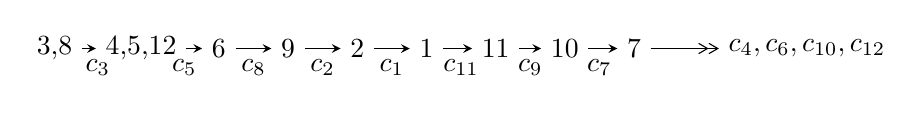
\begin{tikzpicture}[x=25pt, y=7pt]
	% node
	\node (A0) at (-1/8, 0) {3,8};
	\node (A1) at (9/8, 0) {4,5,12};
	\node (A2) at (9/4, 0) {6};
	\node (A3) at (13/4, 0) {9};
	\node (A4) at (17/4, 0) {2};
	\node (A5) at (21/4, 0) {1};
	\node (A6) at (25/4, 0) {11};
	\node (A7) at (29/4, 0) {10};
	\node (A8) at (33/4, 0) {7};
	\node (C1) at (1/2, -1) {$c_{3}$};
	\node (C2) at (7/4, -1) {$c_{5}$};
	\node (C3) at (11/4, -1) {$c_{8}$};
	\node (C4) at (15/4, -1) {$c_{2}$};
	\node (C5) at (19/4, -1) {$c_{1}$};
	\node (C6) at (23/4, -1) {$c_{11}$};
	\node (C7) at (27/4, -1) {$c_{9}$};
	\node (C8) at (31/4, -1) {$c_{7}$};
	\node (A9) at (43/4, 0) {$c_{4},c_{6},c_{10},c_{12}$};

	% edge
	\draw[->,>=stealth]	
	(A0) edge (A1) (A1) edge (A2) (A2) edge (A3) (A3) edge (A4) (A4) edge (A5) (A5) edge (A6) (A6) edge (A7) (A7) edge (A8) ;
	\draw[->>,>={angle 60}]	
	(A8) edge (A9);
\end{tikzpicture} \\ 

\end{tabular} \\

\footnotetext{
The image of knot diagram is generated by the software ``\textbf{Draw programme}" developed by Andrew Bartholomew(\url{http://www.layer8.co.uk/maths/draw/index.htm\#Running-draw}), where we modified some parts for our purpose(\url{https://github.com/CATsTAILs/LinksPainter}).
}\phantom \\ \newline 
\centering \textbf{Ideals for irreducible components\footnotemark of $X_{\text{par}}$} 
 
\begin{align*}
I^u_{1}&=\langle 
-2.85904\times10^{163} u^{70}-4.35691\times10^{163} u^{69}+\cdots+1.78033\times10^{166} d+6.66454\times10^{165},\\
\phantom{I^u_{1}}&\phantom{= \langle  }6.92432\times10^{163} u^{70}+3.87141\times10^{164} u^{69}+\cdots+1.42427\times10^{167} c-4.02166\times10^{167},\\
\phantom{I^u_{1}}&\phantom{= \langle  }-3.44890\times10^{145} u^{70}-6.44692\times10^{145} u^{69}+\cdots+2.51636\times10^{148} b-3.51686\times10^{147},\\
\phantom{I^u_{1}}&\phantom{= \langle  }2.31798\times10^{146} u^{70}+5.72081\times10^{146} u^{69}+\cdots+1.00654\times10^{149} a-4.30269\times10^{149},\\
\phantom{I^u_{1}}&\phantom{= \langle  }u^{71}+2 u^{70}+\cdots-1536 u^2+512\rangle \\
I^u_{2}&=\langle 
d,\;c-1,\;- a^2 u^2+b+2 a-2,\;2 u^8 a^2-3 u^8 a+\cdots+3 a-1,\;u^9- u^8-2 u^7+3 u^6+u^5-3 u^4+2 u^3- u+1\rangle \\
\\
I^v_{1}&=\langle 
c,\;d-1,\;b,\;a-1,\;v^2- v+1\rangle \\
I^v_{2}&=\langle 
a,\;d+1,\;c+a,\;b-1,\;v^2+v+1\rangle \\
I^v_{3}&=\langle 
a,\;d,\;c-1,\;b-1,\;v-1\rangle \\
I^v_{4}&=\langle 
a,\;d^2 v^2+d v+1,\;v^2 d c- v^2 d+c v+a- v,\;d a- c+1,\;c^2 v^2+c a v-2 v^2 c+a^2- a v+v^2,\;b-1\rangle \\
\end{align*}
\raggedright * 5 irreducible components of $\dim_{\mathbb{C}}=0$, with total 103 representations.\\
\raggedright * 1 irreducible components of $\dim_{\mathbb{C}}=1$ \\
\footnotetext{All coefficients of polynomials are rational numbers. But the coefficients are sometimes approximated in decimal forms when there is not enough margin.}
\newpage
\renewcommand{\arraystretch}{1}
\centering \section*{I. $I^u_{1}= \langle -2.86\times10^{163} u^{70}-4.36\times10^{163} u^{69}+\cdots+1.78\times10^{166} d+6.66\times10^{165},\;6.92\times10^{163} u^{70}+3.87\times10^{164} u^{69}+\cdots+1.42\times10^{167} c-4.02\times10^{167},\;-3.45\times10^{145} u^{70}-6.45\times10^{145} u^{69}+\cdots+2.52\times10^{148} b-3.52\times10^{147},\;2.32\times10^{146} u^{70}+5.72\times10^{146} u^{69}+\cdots+1.01\times10^{149} a-4.30\times10^{149},\;u^{71}+2 u^{70}+\cdots-1536 u^2+512 \rangle$}
\flushleft \textbf{(i) Arc colorings}\\
\begin{tabular}{m{7pt} m{180pt} m{7pt} m{180pt} }
\flushright $a_{3}=$&$\begin{pmatrix}1\\0\end{pmatrix}$ \\
\flushright $a_{8}=$&$\begin{pmatrix}0\\u\end{pmatrix}$ \\
\flushright $a_{4}=$&$\begin{pmatrix}1\\- u^2\end{pmatrix}$ \\
\flushright $a_{5}=$&$\begin{pmatrix}-0.00230291 u^{70}-0.00568363 u^{69}+\cdots+2.16416 u+4.27473\\0.00137059 u^{70}+0.00256201 u^{69}+\cdots-0.903349 u+0.139760\end{pmatrix}$ \\
\flushright $a_{12}=$&$\begin{pmatrix}-0.000486167 u^{70}-0.00271817 u^{69}+\cdots+1.59401 u+2.82367\\0.00160590 u^{70}+0.00244724 u^{69}+\cdots-0.182976 u-0.374342\end{pmatrix}$ \\
\flushright $a_{6}=$&$\begin{pmatrix}-0.00198935 u^{70}-0.00509444 u^{69}+\cdots+1.69724 u+3.40383\\-0.000342331 u^{70}-0.000350145 u^{69}+\cdots-0.477053 u-0.323800\end{pmatrix}$ \\
\flushright $a_{9}=$&$\begin{pmatrix}u\\- u^3+u\end{pmatrix}$ \\
\flushright $a_{2}=$&$\begin{pmatrix}-0.00230291 u^{70}-0.00568363 u^{69}+\cdots+2.16416 u+4.27473\\0.000610137 u^{70}+0.000608739 u^{69}+\cdots-0.275743 u-0.691592\end{pmatrix}$ \\
\flushright $a_{1}=$&$\begin{pmatrix}-0.00169278 u^{70}-0.00507489 u^{69}+\cdots+1.88842 u+3.58313\\0.000610137 u^{70}+0.000608739 u^{69}+\cdots-0.275743 u-0.691592\end{pmatrix}$ \\
\flushright $a_{11}=$&$\begin{pmatrix}0.000942281 u^{70}-0.000435385 u^{69}+\cdots+0.824718 u+2.36850\\0.00186115 u^{70}+0.00285291 u^{69}+\cdots-0.220899 u-1.12345\end{pmatrix}$ \\
\flushright $a_{10}=$&$\begin{pmatrix}0.000964925 u^{70}+0.00251480 u^{69}+\cdots-0.510969 u-0.979894\\-0.00121332 u^{70}-0.00285890 u^{69}+\cdots+0.588206 u+1.41140\end{pmatrix}$ \\
\flushright $a_{7}=$&$\begin{pmatrix}-0.00150252 u^{70}-0.00389403 u^{69}+\cdots+1.52807 u+2.30414\\-0.00101635 u^{70}-0.00117586 u^{69}+\cdots-0.0659421 u-0.519527\end{pmatrix}$\\&\end{tabular}
\flushleft \textbf{(ii) Obstruction class $= -1$}\\~\\
\flushleft \textbf{(iii) Cusp Shapes $= 0.000644196 u^{70}-0.0111115 u^{69}+\cdots+0.863041 u+15.1191$}\\~\\
\newpage\renewcommand{\arraystretch}{1}
\flushleft \textbf{(iv) u-Polynomials at the component}\newline \\
\begin{tabular}{m{50pt}|m{274pt}}
Crossings & \hspace{64pt}u-Polynomials at each crossing \\
\hline $$\begin{aligned}c_{1}\end{aligned}$$&$\begin{aligned}
&u^{71}+30 u^{70}+\cdots+4640 u+256
\end{aligned}$\\
\hline $$\begin{aligned}c_{2},c_{4}\end{aligned}$$&$\begin{aligned}
&u^{71}-8 u^{70}+\cdots+56 u-16
\end{aligned}$\\
\hline $$\begin{aligned}c_{3},c_{8}\end{aligned}$$&$\begin{aligned}
&u^{71}-2 u^{70}+\cdots+1536 u^2-512
\end{aligned}$\\
\hline $$\begin{aligned}c_{5},c_{6},c_{12}\end{aligned}$$&$\begin{aligned}
&u^{71}+8 u^{70}+\cdots+56 u-16
\end{aligned}$\\
\hline $$\begin{aligned}c_{7},c_{10}\end{aligned}$$&$\begin{aligned}
&u^{71}+2 u^{70}+\cdots-5 u^2-4
\end{aligned}$\\
\hline $$\begin{aligned}c_{9},c_{11}\end{aligned}$$&$\begin{aligned}
&u^{71}+24 u^{70}+\cdots-40 u-16
\end{aligned}$\\
\hline
\end{tabular}\\~\\
\newpage\renewcommand{\arraystretch}{1}
\flushleft \textbf{(v) Riley Polynomials at the component}\newline \\
\begin{tabular}{m{50pt}|m{274pt}}
Crossings & \hspace{64pt}Riley Polynomials at each crossing \\
\hline $$\begin{aligned}c_{1}\end{aligned}$$&$\begin{aligned}
&y^{71}+30 y^{70}+\cdots+5022208 y-65536
\end{aligned}$\\
\hline $$\begin{aligned}c_{2},c_{4}\end{aligned}$$&$\begin{aligned}
&y^{71}-30 y^{70}+\cdots+4640 y-256
\end{aligned}$\\
\hline $$\begin{aligned}c_{3},c_{8}\end{aligned}$$&$\begin{aligned}
&y^{71}-30 y^{70}+\cdots+1572864 y-262144
\end{aligned}$\\
\hline $$\begin{aligned}c_{5},c_{6},c_{12}\end{aligned}$$&$\begin{aligned}
&y^{71}-70 y^{70}+\cdots-1504 y-256
\end{aligned}$\\
\hline $$\begin{aligned}c_{7},c_{10}\end{aligned}$$&$\begin{aligned}
&y^{71}+24 y^{70}+\cdots-40 y-16
\end{aligned}$\\
\hline $$\begin{aligned}c_{9},c_{11}\end{aligned}$$&$\begin{aligned}
&y^{71}+48 y^{70}+\cdots-6880 y-256
\end{aligned}$\\
\hline
\end{tabular}\\~\\
\newpage\flushleft \textbf{(vi) Complex Volumes and Cusp Shapes}
$$\begin{array}{c|c|c}  
\text{Solutions to }I^u_{1}& \I (\text{vol} + \sqrt{-1}CS) & \text{Cusp shape}\\
 \hline 
\begin{aligned}
u &= \phantom{-}0.372595 + 0.922213 I \\
a &= \phantom{-}0.485748 - 0.116000 I \\
b &= \phantom{-}0.947611 + 0.465102 I \\
c &= -0.384570 - 0.910845 I \\
d &= -0.352109 - 0.909932 I\end{aligned}
 & -0.206074 - 1.106620 I & \phantom{-}1.82615 + 2.10157 I \\ \hline\begin{aligned}
u &= \phantom{-}0.372595 - 0.922213 I \\
a &= \phantom{-}0.485748 + 0.116000 I \\
b &= \phantom{-}0.947611 - 0.465102 I \\
c &= -0.384570 + 0.910845 I \\
d &= -0.352109 + 0.909932 I\end{aligned}
 & -0.206074 + 1.106620 I & \phantom{-}1.82615 - 2.10157 I \\ \hline\begin{aligned}
u &= -0.661751 + 0.731261 I \\
a &= \phantom{-}0.455879 + 0.075380 I \\
b &= \phantom{-}1.135190 - 0.353055 I \\
c &= -0.541629 + 0.798372 I \\
d &= -0.648241 + 1.044530 I\end{aligned}
 & -5.31233 + 1.23150 I & -6.16629 - 0.79467 I \\ \hline\begin{aligned}
u &= -0.661751 - 0.731261 I \\
a &= \phantom{-}0.455879 - 0.075380 I \\
b &= \phantom{-}1.135190 + 0.353055 I \\
c &= -0.541629 - 0.798372 I \\
d &= -0.648241 - 1.044530 I\end{aligned}
 & -5.31233 - 1.23150 I & -6.16629 + 0.79467 I \\ \hline\begin{aligned}
u &= -0.216094 + 0.961248 I \\
a &= \phantom{-}0.507916 + 0.138278 I \\
b &= \phantom{-}0.832973 - 0.499020 I \\
c &= \phantom{-}0.383038 - 1.211050 I \\
d &= \phantom{-}1.32096 - 2.52250 I\end{aligned}
 & \phantom{-}2.60149 + 2.06138 I & \phantom{-}6.60052 - 3.22142 I \\ \hline\begin{aligned}
u &= -0.216094 - 0.961248 I \\
a &= \phantom{-}0.507916 - 0.138278 I \\
b &= \phantom{-}0.832973 + 0.499020 I \\
c &= \phantom{-}0.383038 + 1.211050 I \\
d &= \phantom{-}1.32096 + 2.52250 I\end{aligned}
 & \phantom{-}2.60149 - 2.06138 I & \phantom{-}6.60052 + 3.22142 I\\
 \hline 
 \end{array}$$\newpage$$\begin{array}{c|c|c}  
\text{Solutions to }I^u_{1}& \I (\text{vol} + \sqrt{-1}CS) & \text{Cusp shape}\\
 \hline 
\begin{aligned}
u &= \phantom{-}0.510340 + 0.919175 I \\
a &= \phantom{-}0.466316 - 0.105830 I \\
b &= \phantom{-}1.039430 + 0.462844 I \\
c &= \phantom{-}0.06669 + 1.49411 I \\
d &= \phantom{-}0.71893 + 3.03674 I\end{aligned}
 & -1.22762 - 4.53498 I & -0.48837 + 4.83158 I \\ \hline\begin{aligned}
u &= \phantom{-}0.510340 - 0.919175 I \\
a &= \phantom{-}0.466316 + 0.105830 I \\
b &= \phantom{-}1.039430 - 0.462844 I \\
c &= \phantom{-}0.06669 - 1.49411 I \\
d &= \phantom{-}0.71893 - 3.03674 I\end{aligned}
 & -1.22762 + 4.53498 I & -0.48837 - 4.83158 I \\ \hline\begin{aligned}
u &= -0.843761 + 0.417994 I \\
a &= \phantom{-}0.442312 + 0.038598 I \\
b &= \phantom{-}1.243760 - 0.195802 I \\
c &= -0.734788 + 0.784462 I \\
d &= -1.01432 + 1.24587 I\end{aligned}
 & -1.74336 - 3.95563 I & \phantom{-}0.57229 + 6.63484 I \\ \hline\begin{aligned}
u &= -0.843761 - 0.417994 I \\
a &= \phantom{-}0.442312 - 0.038598 I \\
b &= \phantom{-}1.243760 + 0.195802 I \\
c &= -0.734788 - 0.784462 I \\
d &= -1.01432 - 1.24587 I\end{aligned}
 & -1.74336 + 3.95563 I & \phantom{-}0.57229 - 6.63484 I \\ \hline\begin{aligned}
u &= \phantom{-}0.980094 + 0.401535 I \\
a &= \phantom{-}0.12281 - 1.97463 I \\
b &= -0.968625 + 0.504474 I \\
c &= -1.197140 - 0.714849 I \\
d &= -0.337051 + 0.964290 I\end{aligned}
 & \phantom{-}0.13020 + 4.00402 I & \phantom{-}4.41276 - 6.69495 I \\ \hline\begin{aligned}
u &= \phantom{-}0.980094 - 0.401535 I \\
a &= \phantom{-}0.12281 + 1.97463 I \\
b &= -0.968625 - 0.504474 I \\
c &= -1.197140 + 0.714849 I \\
d &= -0.337051 - 0.964290 I\end{aligned}
 & \phantom{-}0.13020 - 4.00402 I & \phantom{-}4.41276 + 6.69495 I\\
 \hline 
 \end{array}$$\newpage$$\begin{array}{c|c|c}  
\text{Solutions to }I^u_{1}& \I (\text{vol} + \sqrt{-1}CS) & \text{Cusp shape}\\
 \hline 
\begin{aligned}
u &= -0.482781 + 0.984718 I \\
a &= \phantom{-}0.465372 + 0.116264 I \\
b &= \phantom{-}1.022580 - 0.505302 I \\
c &= -0.456078 + 0.912887 I \\
d &= -0.380030 + 1.013380 I\end{aligned}
 & -0.99233 + 6.45679 I & \phantom{-}0.34368 - 6.97496 I \\ \hline\begin{aligned}
u &= -0.482781 - 0.984718 I \\
a &= \phantom{-}0.465372 - 0.116264 I \\
b &= \phantom{-}1.022580 + 0.505302 I \\
c &= -0.456078 - 0.912887 I \\
d &= -0.380030 - 1.013380 I\end{aligned}
 & -0.99233 - 6.45679 I & \phantom{-}0.34368 + 6.97496 I \\ \hline\begin{aligned}
u &= -0.777198 + 0.427799 I \\
a &= \phantom{-}0.07067 + 2.71633 I \\
b &= -0.990428 - 0.367895 I \\
c &= -1.55052 + 1.42781 I \\
d &= -0.496780 - 0.852703 I\end{aligned}
 & -1.94652 + 0.34051 I & -0.37051 + 3.03065 I \\ \hline\begin{aligned}
u &= -0.777198 - 0.427799 I \\
a &= \phantom{-}0.07067 - 2.71633 I \\
b &= -0.990428 + 0.367895 I \\
c &= -1.55052 - 1.42781 I \\
d &= -0.496780 + 0.852703 I\end{aligned}
 & -1.94652 - 0.34051 I & -0.37051 - 3.03065 I \\ \hline\begin{aligned}
u &= -1.127060 + 0.152551 I \\
a &= \phantom{-}0.625091 - 1.046840 I \\
b &= -0.579522 + 0.704176 I \\
c &= -2.04566 + 1.44271 I \\
d &= \phantom{-}1.04128 - 1.78221 I\end{aligned}
 & \phantom{-}4.50468 + 2.47836 I & \phantom{-}7.49354 - 3.38416 I \\ \hline\begin{aligned}
u &= -1.127060 - 0.152551 I \\
a &= \phantom{-}0.625091 + 1.046840 I \\
b &= -0.579522 - 0.704176 I \\
c &= -2.04566 - 1.44271 I \\
d &= \phantom{-}1.04128 + 1.78221 I\end{aligned}
 & \phantom{-}4.50468 - 2.47836 I & \phantom{-}7.49354 + 3.38416 I\\
 \hline 
 \end{array}$$\newpage$$\begin{array}{c|c|c}  
\text{Solutions to }I^u_{1}& \I (\text{vol} + \sqrt{-1}CS) & \text{Cusp shape}\\
 \hline 
\begin{aligned}
u &= -0.982347 + 0.611518 I \\
a &= -0.39397 + 1.91571 I \\
b &= -1.102990 - 0.500818 I \\
c &= -1.67667 + 0.41013 I \\
d &= -0.438066 - 1.090250 I\end{aligned}
 & -4.29573 - 6.37313 I & -3.00781 + 7.19219 I \\ \hline\begin{aligned}
u &= -0.982347 - 0.611518 I \\
a &= -0.39397 - 1.91571 I \\
b &= -1.102990 + 0.500818 I \\
c &= -1.67667 - 0.41013 I \\
d &= -0.438066 + 1.090250 I\end{aligned}
 & -4.29573 + 6.37313 I & -3.00781 - 7.19219 I \\ \hline\begin{aligned}
u &= -1.173990 + 0.222972 I \\
a &= \phantom{-}0.579369 - 0.967956 I \\
b &= -0.544738 + 0.760609 I \\
c &= -0.311368 - 0.051508 I \\
d &= \phantom{-}0.148549 + 1.017150 I\end{aligned}
 & \phantom{-}5.09577 - 1.83902 I & \phantom{-}8.24819 + 0. I\phantom{ +0.000000I} \\ \hline\begin{aligned}
u &= -1.173990 - 0.222972 I \\
a &= \phantom{-}0.579369 + 0.967956 I \\
b &= -0.544738 - 0.760609 I \\
c &= -0.311368 + 0.051508 I \\
d &= \phantom{-}0.148549 - 1.017150 I\end{aligned}
 & \phantom{-}5.09577 + 1.83902 I & \phantom{-}8.24819 + 0. I\phantom{ +0.000000I} \\ \hline\begin{aligned}
u &= \phantom{-}1.203430 + 0.094057 I \\
a &= \phantom{-}0.526070 + 1.096070 I \\
b &= -0.644095 - 0.741530 I \\
c &= -0.422317 + 0.128209 I \\
d &= \phantom{-}0.061447 - 1.014150 I\end{aligned}
 & \phantom{-}5.36659 - 3.89584 I & \phantom{-}8.41567 + 5.55146 I \\ \hline\begin{aligned}
u &= \phantom{-}1.203430 - 0.094057 I \\
a &= \phantom{-}0.526070 - 1.096070 I \\
b &= -0.644095 + 0.741530 I \\
c &= -0.422317 - 0.128209 I \\
d &= \phantom{-}0.061447 + 1.014150 I\end{aligned}
 & \phantom{-}5.36659 + 3.89584 I & \phantom{-}8.41567 - 5.55146 I\\
 \hline 
 \end{array}$$\newpage$$\begin{array}{c|c|c}  
\text{Solutions to }I^u_{1}& \I (\text{vol} + \sqrt{-1}CS) & \text{Cusp shape}\\
 \hline 
\begin{aligned}
u &= -1.117530 + 0.478181 I \\
a &= \phantom{-}0.592431 - 0.750598 I \\
b &= -0.352089 + 0.820889 I \\
c &= -2.11325 + 0.00351 I \\
d &= \phantom{-}0.82348 - 1.49852 I\end{aligned}
 & \phantom{-}3.15531 - 5.12152 I & \phantom{-0.000000 } 0 \\ \hline\begin{aligned}
u &= -1.117530 - 0.478181 I \\
a &= \phantom{-}0.592431 + 0.750598 I \\
b &= -0.352089 - 0.820889 I \\
c &= -2.11325 - 0.00351 I \\
d &= \phantom{-}0.82348 + 1.49852 I\end{aligned}
 & \phantom{-}3.15531 + 5.12152 I & \phantom{-0.000000 } 0 \\ \hline\begin{aligned}
u &= \phantom{-}1.137650 + 0.460214 I \\
a &= -0.04379 - 1.65202 I \\
b &= -1.016040 + 0.604894 I \\
c &= \phantom{-}1.76875 + 1.86712 I \\
d &= \phantom{-}0.70340 - 2.59306 I\end{aligned}
 & \phantom{-}3.19656 + 2.55854 I & \phantom{-0.000000 } 0 \\ \hline\begin{aligned}
u &= \phantom{-}1.137650 - 0.460214 I \\
a &= -0.04379 + 1.65202 I \\
b &= -1.016040 - 0.604894 I \\
c &= \phantom{-}1.76875 - 1.86712 I \\
d &= \phantom{-}0.70340 + 2.59306 I\end{aligned}
 & \phantom{-}3.19656 - 2.55854 I & \phantom{-0.000000 } 0 \\ \hline\begin{aligned}
u &= \phantom{-}0.725491 + 0.260568 I \\
a &= \phantom{-}0.454620 - 0.024037 I \\
b &= \phantom{-}1.193510 + 0.115977 I \\
c &= -0.858903 - 0.665057 I \\
d &= -1.33178 - 1.09391 I\end{aligned}
 & -1.09934 - 1.05821 I & \phantom{-}3.09814 - 1.72718 I \\ \hline\begin{aligned}
u &= \phantom{-}0.725491 - 0.260568 I \\
a &= \phantom{-}0.454620 + 0.024037 I \\
b &= \phantom{-}1.193510 - 0.115977 I \\
c &= -0.858903 + 0.665057 I \\
d &= -1.33178 + 1.09391 I\end{aligned}
 & -1.09934 + 1.05821 I & \phantom{-}3.09814 + 1.72718 I\\
 \hline 
 \end{array}$$\newpage$$\begin{array}{c|c|c}  
\text{Solutions to }I^u_{1}& \I (\text{vol} + \sqrt{-1}CS) & \text{Cusp shape}\\
 \hline 
\begin{aligned}
u &= \phantom{-}0.247645 + 1.226350 I \\
a &= \phantom{-}0.509066 + 0.265043 I \\
b &= \phantom{-}0.545453 - 0.804634 I \\
c &= \phantom{-}0.148746 - 0.746604 I \\
d &= \phantom{-}0.89036 - 1.73101 I\end{aligned}
 & \phantom{-}6.94619 + 1.12108 I & \phantom{-0.000000 } 0 \\ \hline\begin{aligned}
u &= \phantom{-}0.247645 - 1.226350 I \\
a &= \phantom{-}0.509066 - 0.265043 I \\
b &= \phantom{-}0.545453 + 0.804634 I \\
c &= \phantom{-}0.148746 + 0.746604 I \\
d &= \phantom{-}0.89036 + 1.73101 I\end{aligned}
 & \phantom{-}6.94619 - 1.12108 I & \phantom{-0.000000 } 0 \\ \hline\begin{aligned}
u &= -0.464983 + 0.581438 I \\
a &= \phantom{-}0.788881 - 0.333426 I \\
b &= \phantom{-}0.075493 + 0.454564 I \\
c &= \phantom{-}0.323459 + 0.239200 I \\
d &= \phantom{-}0.936440 + 0.862765 I\end{aligned}
 & \phantom{-}1.011140 + 0.938516 I & \phantom{-}3.66296 + 0.79830 I \\ \hline\begin{aligned}
u &= -0.464983 - 0.581438 I \\
a &= \phantom{-}0.788881 + 0.333426 I \\
b &= \phantom{-}0.075493 - 0.454564 I \\
c &= \phantom{-}0.323459 - 0.239200 I \\
d &= \phantom{-}0.936440 - 0.862765 I\end{aligned}
 & \phantom{-}1.011140 - 0.938516 I & \phantom{-}3.66296 - 0.79830 I \\ \hline\begin{aligned}
u &= -0.368570 + 1.210560 I \\
a &= \phantom{-}0.515481 - 0.295559 I \\
b &= \phantom{-}0.459973 + 0.837098 I \\
c &= \phantom{-}0.122518 + 0.676794 I \\
d &= \phantom{-}0.83963 + 1.62701 I\end{aligned}
 & \phantom{-}6.42018 + 4.68044 I & \phantom{-0.000000 } 0 \\ \hline\begin{aligned}
u &= -0.368570 - 1.210560 I \\
a &= \phantom{-}0.515481 + 0.295559 I \\
b &= \phantom{-}0.459973 - 0.837098 I \\
c &= \phantom{-}0.122518 - 0.676794 I \\
d &= \phantom{-}0.83963 - 1.62701 I\end{aligned}
 & \phantom{-}6.42018 - 4.68044 I & \phantom{-0.000000 } 0\\
 \hline 
 \end{array}$$\newpage$$\begin{array}{c|c|c}  
\text{Solutions to }I^u_{1}& \I (\text{vol} + \sqrt{-1}CS) & \text{Cusp shape}\\
 \hline 
\begin{aligned}
u &= \phantom{-}1.248660 + 0.306382 I \\
a &= \phantom{-}0.516438 + 0.892389 I \\
b &= -0.514200 - 0.839448 I \\
c &= -1.73216 - 0.62281 I \\
d &= \phantom{-}0.84440 + 1.69272 I\end{aligned}
 & \phantom{-}7.51654 + 1.91781 I & \phantom{-0.000000 } 0 \\ \hline\begin{aligned}
u &= \phantom{-}1.248660 - 0.306382 I \\
a &= \phantom{-}0.516438 - 0.892389 I \\
b &= -0.514200 + 0.839448 I \\
c &= -1.73216 + 0.62281 I \\
d &= \phantom{-}0.84440 - 1.69272 I\end{aligned}
 & \phantom{-}7.51654 - 1.91781 I & \phantom{-0.000000 } 0 \\ \hline\begin{aligned}
u &= -0.504947 + 1.215580 I \\
a &= \phantom{-}0.443142 + 0.140469 I \\
b &= \phantom{-}1.050580 - 0.650000 I \\
c &= -0.011223 - 1.220060 I \\
d &= \phantom{-}0.60444 - 2.51848 I\end{aligned}
 & \phantom{-}5.42990 + 4.32973 I & \phantom{-0.000000 } 0 \\ \hline\begin{aligned}
u &= -0.504947 - 1.215580 I \\
a &= \phantom{-}0.443142 - 0.140469 I \\
b &= \phantom{-}1.050580 + 0.650000 I \\
c &= -0.011223 + 1.220060 I \\
d &= \phantom{-}0.60444 + 2.51848 I\end{aligned}
 & \phantom{-}5.42990 - 4.32973 I & \phantom{-0.000000 } 0 \\ \hline\begin{aligned}
u &= \phantom{-}1.152900 + 0.667545 I \\
a &= -0.37747 - 1.57567 I \\
b &= -1.143790 + 0.600204 I \\
c &= \phantom{-}2.23046 + 0.59659 I \\
d &= \phantom{-}0.41994 - 2.63177 I\end{aligned}
 & \phantom{-}0.80414 + 10.42400 I & \phantom{-0.000000 } 0 \\ \hline\begin{aligned}
u &= \phantom{-}1.152900 - 0.667545 I \\
a &= -0.37747 + 1.57567 I \\
b &= -1.143790 - 0.600204 I \\
c &= \phantom{-}2.23046 - 0.59659 I \\
d &= \phantom{-}0.41994 + 2.63177 I\end{aligned}
 & \phantom{-}0.80414 - 10.42400 I & \phantom{-0.000000 } 0\\
 \hline 
 \end{array}$$\newpage$$\begin{array}{c|c|c}  
\text{Solutions to }I^u_{1}& \I (\text{vol} + \sqrt{-1}CS) & \text{Cusp shape}\\
 \hline 
\begin{aligned}
u &= \phantom{-}1.185800 + 0.609579 I \\
a &= -0.27825 - 1.55393 I \\
b &= -1.111650 + 0.623537 I \\
c &= -1.371570 - 0.115410 I \\
d &= -0.331493 + 1.161530 I\end{aligned}
 & \phantom{-}2.33908 + 6.73341 I & \phantom{-0.000000 } 0 \\ \hline\begin{aligned}
u &= \phantom{-}1.185800 - 0.609579 I \\
a &= -0.27825 + 1.55393 I \\
b &= -1.111650 - 0.623537 I \\
c &= -1.371570 + 0.115410 I \\
d &= -0.331493 - 1.161530 I\end{aligned}
 & \phantom{-}2.33908 - 6.73341 I & \phantom{-0.000000 } 0 \\ \hline\begin{aligned}
u &= \phantom{-}0.593784 + 1.208600 I \\
a &= \phantom{-}0.435237 - 0.132054 I \\
b &= \phantom{-}1.103920 + 0.638344 I \\
c &= -0.064916 + 1.245600 I \\
d &= \phantom{-}0.50321 + 2.55667 I\end{aligned}
 & \phantom{-}4.48821 - 10.17210 I & \phantom{-0.000000 } 0 \\ \hline\begin{aligned}
u &= \phantom{-}0.593784 - 1.208600 I \\
a &= \phantom{-}0.435237 + 0.132054 I \\
b &= \phantom{-}1.103920 - 0.638344 I \\
c &= -0.064916 - 1.245600 I \\
d &= \phantom{-}0.50321 - 2.55667 I\end{aligned}
 & \phantom{-}4.48821 + 10.17210 I & \phantom{-0.000000 } 0 \\ \hline\begin{aligned}
u &= -1.233000 + 0.545251 I \\
a &= -0.17535 + 1.50144 I \\
b &= -1.076740 - 0.657064 I \\
c &= \phantom{-}1.59832 - 1.09061 I \\
d &= \phantom{-}0.55162 + 2.51495 I\end{aligned}
 & \phantom{-}5.82408 - 7.48275 I & \phantom{-0.000000 } 0 \\ \hline\begin{aligned}
u &= -1.233000 - 0.545251 I \\
a &= -0.17535 - 1.50144 I \\
b &= -1.076740 + 0.657064 I \\
c &= \phantom{-}1.59832 + 1.09061 I \\
d &= \phantom{-}0.55162 - 2.51495 I\end{aligned}
 & \phantom{-}5.82408 + 7.48275 I & \phantom{-0.000000 } 0\\
 \hline 
 \end{array}$$\newpage$$\begin{array}{c|c|c}  
\text{Solutions to }I^u_{1}& \I (\text{vol} + \sqrt{-1}CS) & \text{Cusp shape}\\
 \hline 
\begin{aligned}
u &= \phantom{-}0.176438 + 0.617781 I \\
a &= \phantom{-}0.536936 - 0.059094 I \\
b &= \phantom{-}0.840129 + 0.202520 I \\
c &= \phantom{-}1.43629 + 1.69472 I \\
d &= \phantom{-}3.37169 + 3.42725 I\end{aligned}
 & \phantom{-}0.42738 + 1.60074 I & \phantom{-}0.77404 - 2.18898 I \\ \hline\begin{aligned}
u &= \phantom{-}0.176438 - 0.617781 I \\
a &= \phantom{-}0.536936 + 0.059094 I \\
b &= \phantom{-}0.840129 - 0.202520 I \\
c &= \phantom{-}1.43629 - 1.69472 I \\
d &= \phantom{-}3.37169 - 3.42725 I\end{aligned}
 & \phantom{-}0.42738 - 1.60074 I & \phantom{-}0.77404 + 2.18898 I \\ \hline\begin{aligned}
u &= -1.181300 + 0.680585 I \\
a &= -0.38029 + 1.52881 I \\
b &= -1.153230 - 0.615988 I \\
c &= -1.45518 + 0.03477 I \\
d &= -0.355666 - 1.191500 I\end{aligned}
 & \phantom{-}1.22414 - 12.55690 I & \phantom{-0.000000 } 0 \\ \hline\begin{aligned}
u &= -1.181300 - 0.680585 I \\
a &= -0.38029 - 1.52881 I \\
b &= -1.153230 + 0.615988 I \\
c &= -1.45518 - 0.03477 I \\
d &= -0.355666 + 1.191500 I\end{aligned}
 & \phantom{-}1.22414 + 12.55690 I & \phantom{-0.000000 } 0 \\ \hline\begin{aligned}
u &= -0.010891 + 0.626888 I \\
a &= \phantom{-}0.651032 - 0.036187 I \\
b &= \phantom{-}0.531292 + 0.085114 I \\
c &= \phantom{-}1.184550 - 0.522827 I \\
d &= \phantom{-}0.081339 - 0.143491 I\end{aligned}
 & \phantom{-}0.65592 - 2.35939 I & \phantom{-}1.51759 + 4.85897 I \\ \hline\begin{aligned}
u &= -0.010891 - 0.626888 I \\
a &= \phantom{-}0.651032 + 0.036187 I \\
b &= \phantom{-}0.531292 - 0.085114 I \\
c &= \phantom{-}1.184550 + 0.522827 I \\
d &= \phantom{-}0.081339 + 0.143491 I\end{aligned}
 & \phantom{-}0.65592 + 2.35939 I & \phantom{-}1.51759 - 4.85897 I\\
 \hline 
 \end{array}$$\newpage$$\begin{array}{c|c|c}  
\text{Solutions to }I^u_{1}& \I (\text{vol} + \sqrt{-1}CS) & \text{Cusp shape}\\
 \hline 
\begin{aligned}
u &= \phantom{-}0.617428 + 0.085193 I \\
a &= \phantom{-}2.98131 - 1.84944 I \\
b &= -0.757787 + 0.150255 I \\
c &= \phantom{-}1.27420 - 1.43204 I \\
d &= -0.305853 + 0.300706 I\end{aligned}
 & -0.93328 + 2.67780 I & \phantom{-}3.99337 - 7.95500 I \\ \hline\begin{aligned}
u &= \phantom{-}0.617428 - 0.085193 I \\
a &= \phantom{-}2.98131 + 1.84944 I \\
b &= -0.757787 - 0.150255 I \\
c &= \phantom{-}1.27420 + 1.43204 I \\
d &= -0.305853 - 0.300706 I\end{aligned}
 & -0.93328 - 2.67780 I & \phantom{-}3.99337 + 7.95500 I \\ \hline\begin{aligned}
u &= -0.591164\phantom{ +0.000000I} \\
a &= \phantom{-}1.74742\phantom{ +0.000000I} \\
b &= -0.427729\phantom{ +0.000000I} \\
c &= \phantom{-}0.644601\phantom{ +0.000000I} \\
d &= \phantom{-}0.251389\phantom{ +0.000000I}\end{aligned}
 & \phantom{-}1.02886\phantom{ +0.000000I} & \phantom{-}10.5160\phantom{ +0.000000I} \\ \hline\begin{aligned}
u &= \phantom{-}0.282782 + 0.492299 I \\
a &= \phantom{-}0.508237 - 0.042524 I \\
b &= \phantom{-}0.953908 + 0.163482 I \\
c &= -0.332411 - 0.449116 I \\
d &= -0.705044 - 0.471800 I\end{aligned}
 & -1.67984 - 0.60130 I & -3.90300 + 0.33160 I \\ \hline\begin{aligned}
u &= \phantom{-}0.282782 - 0.492299 I \\
a &= \phantom{-}0.508237 + 0.042524 I \\
b &= \phantom{-}0.953908 - 0.163482 I \\
c &= -0.332411 + 0.449116 I \\
d &= -0.705044 + 0.471800 I\end{aligned}
 & -1.67984 + 0.60130 I & -3.90300 - 0.33160 I \\ \hline\begin{aligned}
u &= \phantom{-}1.33133 + 0.61244 I \\
a &= \phantom{-}0.451627 + 0.707103 I \\
b &= -0.358449 - 1.004460 I \\
c &= -1.50323 + 0.13255 I \\
d &= \phantom{-}0.65119 + 1.56469 I\end{aligned}
 & \phantom{-}10.54930 + 5.35435 I & \phantom{-0.000000 } 0\\
 \hline 
 \end{array}$$\newpage$$\begin{array}{c|c|c}  
\text{Solutions to }I^u_{1}& \I (\text{vol} + \sqrt{-1}CS) & \text{Cusp shape}\\
 \hline 
\begin{aligned}
u &= \phantom{-}1.33133 - 0.61244 I \\
a &= \phantom{-}0.451627 - 0.707103 I \\
b &= -0.358449 + 1.004460 I \\
c &= -1.50323 - 0.13255 I \\
d &= \phantom{-}0.65119 - 1.56469 I\end{aligned}
 & \phantom{-}10.54930 - 5.35435 I & \phantom{-0.000000 } 0 \\ \hline\begin{aligned}
u &= -1.29995 + 0.68416 I \\
a &= \phantom{-}0.458847 - 0.670856 I \\
b &= -0.305396 + 1.015540 I \\
c &= -1.51100 - 0.26879 I \\
d &= \phantom{-}0.62788 - 1.52561 I\end{aligned}
 & \phantom{-}9.4739 - 11.4004 I & \phantom{-0.000000 } 0 \\ \hline\begin{aligned}
u &= -1.29995 - 0.68416 I \\
a &= \phantom{-}0.458847 + 0.670856 I \\
b &= -0.305396 - 1.015540 I \\
c &= -1.51100 + 0.26879 I \\
d &= \phantom{-}0.62788 + 1.52561 I\end{aligned}
 & \phantom{-}9.4739 + 11.4004 I & \phantom{-0.000000 } 0 \\ \hline\begin{aligned}
u &= -1.27239 + 0.75883 I \\
a &= -0.42552 + 1.37781 I \\
b &= -1.204630 - 0.662591 I \\
c &= \phantom{-}1.69978 - 0.12049 I \\
d &= \phantom{-}0.32788 + 2.50055 I\end{aligned}
 & \phantom{-}7.95427 - 11.37060 I & \phantom{-0.000000 } 0 \\ \hline\begin{aligned}
u &= -1.27239 - 0.75883 I \\
a &= -0.42552 - 1.37781 I \\
b &= -1.204630 + 0.662591 I \\
c &= \phantom{-}1.69978 + 0.12049 I \\
d &= \phantom{-}0.32788 - 2.50055 I\end{aligned}
 & \phantom{-}7.95427 + 11.37060 I & \phantom{-0.000000 } 0 \\ \hline\begin{aligned}
u &= \phantom{-}1.24401 + 0.80606 I \\
a &= -0.49137 - 1.37976 I \\
b &= -1.229060 + 0.643191 I \\
c &= \phantom{-}1.80328 - 0.06773 I \\
d &= \phantom{-}0.28176 - 2.52102 I\end{aligned}
 & \phantom{-}6.6365 + 17.3722 I & \phantom{-0.000000 } 0\\
 \hline 
 \end{array}$$\newpage$$\begin{array}{c|c|c}  
\text{Solutions to }I^u_{1}& \I (\text{vol} + \sqrt{-1}CS) & \text{Cusp shape}\\
 \hline 
\begin{aligned}
u &= \phantom{-}1.24401 - 0.80606 I \\
a &= -0.49137 + 1.37976 I \\
b &= -1.229060 - 0.643191 I \\
c &= \phantom{-}1.80328 + 0.06773 I \\
d &= \phantom{-}0.28176 + 2.52102 I\end{aligned}
 & \phantom{-}6.6365 - 17.3722 I & \phantom{-0.000000 } 0 \\ \hline\begin{aligned}
u &= \phantom{-}1.51788 + 0.06429 I \\
a &= \phantom{-}0.205748 - 1.062330 I \\
b &= -0.824278 + 0.907296 I \\
c &= -0.424327 + 0.865938 I \\
d &= \phantom{-}0.67197 - 2.01899 I\end{aligned}
 & \phantom{-}13.78050 + 0.08878 I & \phantom{-0.000000 } 0 \\ \hline\begin{aligned}
u &= \phantom{-}1.51788 - 0.06429 I \\
a &= \phantom{-}0.205748 + 1.062330 I \\
b &= -0.824278 - 0.907296 I \\
c &= -0.424327 - 0.865938 I \\
d &= \phantom{-}0.67197 + 2.01899 I\end{aligned}
 & \phantom{-}13.78050 - 0.08878 I & \phantom{-0.000000 } 0 \\ \hline\begin{aligned}
u &= -1.51414 + 0.16464 I \\
a &= \phantom{-}0.145714 + 1.112210 I \\
b &= -0.884193 - 0.883937 I \\
c &= -0.163454 - 0.908611 I \\
d &= \phantom{-}0.64894 + 2.08801 I\end{aligned}
 & \phantom{-}13.6007 - 6.3599 I & \phantom{-0.000000 } 0 \\ \hline\begin{aligned}
u &= -1.51414 - 0.16464 I \\
a &= \phantom{-}0.145714 - 1.112210 I \\
b &= -0.884193 + 0.883937 I \\
c &= -0.163454 + 0.908611 I \\
d &= \phantom{-}0.64894 - 2.08801 I\end{aligned}
 & \phantom{-}13.6007 + 6.3599 I & \phantom{-0.000000 } 0\\
 \hline 
 \end{array}$$\newpage\newpage\renewcommand{\arraystretch}{1}
\centering \section*{II. $I^u_{2}= \langle d,\;c-1,\;- a^2 u^2+b+2 a-2,\;2 u^8 a^2-3 u^8 a+\cdots+3 a-1,\;u^9- u^8+\cdots- u+1 \rangle$}
\flushleft \textbf{(i) Arc colorings}\\
\begin{tabular}{m{7pt} m{180pt} m{7pt} m{180pt} }
\flushright $a_{3}=$&$\begin{pmatrix}1\\0\end{pmatrix}$ \\
\flushright $a_{8}=$&$\begin{pmatrix}0\\u\end{pmatrix}$ \\
\flushright $a_{4}=$&$\begin{pmatrix}1\\- u^2\end{pmatrix}$ \\
\flushright $a_{5}=$&$\begin{pmatrix}a\\a^2 u^2-2 a+2\end{pmatrix}$ \\
\flushright $a_{12}=$&$\begin{pmatrix}1\\0\end{pmatrix}$ \\
\flushright $a_{6}=$&$\begin{pmatrix}a^2 u^2- a+2\\a^2 u^2-2 a+2\end{pmatrix}$ \\
\flushright $a_{9}=$&$\begin{pmatrix}u\\- u^3+u\end{pmatrix}$ \\
\flushright $a_{2}=$&$\begin{pmatrix}a\\- a^2 u^2- u^2 a+2 a-2\end{pmatrix}$ \\
\flushright $a_{1}=$&$\begin{pmatrix}- a^2 u^2- u^2 a+3 a-2\\- a^2 u^2- u^2 a+2 a-2\end{pmatrix}$ \\
\flushright $a_{11}=$&$\begin{pmatrix}u^4- u^2+1\\- u^6+2 u^4- u^2\end{pmatrix}$ \\
\flushright $a_{10}=$&$\begin{pmatrix}u^7-2 u^5+2 u^3\\- u^8+u^7+3 u^6-2 u^5-3 u^4+2 u^3+1\end{pmatrix}$ \\
\flushright $a_{7}=$&$\begin{pmatrix}- u^2+1\\- u^2\end{pmatrix}$\\&\end{tabular}
\flushleft \textbf{(ii) Obstruction class $= -1$}\\~\\
\flushleft \textbf{(iii) Cusp Shapes $= -4 u^7+8 u^5-4 u^4-8 u^3+4 u^2-4 u+2$}\\~\\
\newpage\renewcommand{\arraystretch}{1}
\flushleft \textbf{(iv) u-Polynomials at the component}\newline \\
\begin{tabular}{m{50pt}|m{274pt}}
Crossings & \hspace{64pt}u-Polynomials at each crossing \\
\hline $$\begin{aligned}c_{1}\end{aligned}$$&$\begin{aligned}
&u^{27}+18 u^{26}+\cdots+5 u+1
\end{aligned}$\\
\hline $$\begin{aligned}c_{2},c_{4},c_{5}\\c_{6},c_{12}\end{aligned}$$&$\begin{aligned}
&u^{27}-9 u^{25}+\cdots- u+1
\end{aligned}$\\
\hline $$\begin{aligned}c_{3},c_{8}\end{aligned}$$&$\begin{aligned}
&(u^9+u^8-2 u^7-3 u^6+u^5+3 u^4+2 u^3- u-1)^3
\end{aligned}$\\
\hline $$\begin{aligned}c_{7},c_{10}\end{aligned}$$&$\begin{aligned}
&(u^9+u^8+2 u^7+u^6+3 u^5+u^4+2 u^3+u-1)^3
\end{aligned}$\\
\hline $$\begin{aligned}c_{9},c_{11}\end{aligned}$$&$\begin{aligned}
&(u^9+3 u^8+8 u^7+13 u^6+17 u^5+17 u^4+12 u^3+6 u^2+u-1)^3
\end{aligned}$\\
\hline
\end{tabular}\\~\\
\newpage\renewcommand{\arraystretch}{1}
\flushleft \textbf{(v) Riley Polynomials at the component}\newline \\
\begin{tabular}{m{50pt}|m{274pt}}
Crossings & \hspace{64pt}Riley Polynomials at each crossing \\
\hline $$\begin{aligned}c_{1}\end{aligned}$$&$\begin{aligned}
&y^{27}-18 y^{26}+\cdots-15 y-1
\end{aligned}$\\
\hline $$\begin{aligned}c_{2},c_{4},c_{5}\\c_{6},c_{12}\end{aligned}$$&$\begin{aligned}
&y^{27}-18 y^{26}+\cdots+5 y-1
\end{aligned}$\\
\hline $$\begin{aligned}c_{3},c_{8}\end{aligned}$$&$\begin{aligned}
&(y^9-5 y^8+12 y^7-15 y^6+9 y^5+y^4-4 y^3+2 y^2+y-1)^3
\end{aligned}$\\
\hline $$\begin{aligned}c_{7},c_{10}\end{aligned}$$&$\begin{aligned}
&(y^9+3 y^8+8 y^7+13 y^6+17 y^5+17 y^4+12 y^3+6 y^2+y-1)^3
\end{aligned}$\\
\hline $$\begin{aligned}c_{9},c_{11}\end{aligned}$$&$\begin{aligned}
&(y^9+7 y^8+20 y^7+25 y^6+5 y^5-15 y^4+22 y^2+13 y-1)^3
\end{aligned}$\\
\hline
\end{tabular}\\~\\
\newpage\flushleft \textbf{(vi) Complex Volumes and Cusp Shapes}
$$\begin{array}{c|c|c}  
\text{Solutions to }I^u_{2}& \I (\text{vol} + \sqrt{-1}CS) & \text{Cusp shape}\\
 \hline 
\begin{aligned}
u &= \phantom{-}0.772920 + 0.510351 I \\
a &= \phantom{-}0.780004 + 0.567068 I \\
b &= -0.161261 - 0.609769 I \\
c &= \phantom{-}1.00000\phantom{ +0.000000I} \\
d &= \phantom{-0.000000 } 0\end{aligned}
 & -1.78344 + 2.09337 I & -0.51499 - 4.16283 I \\ \hline\begin{aligned}
u &= \phantom{-}0.772920 + 0.510351 I \\
a &= \phantom{-}0.448284 - 0.048652 I \\
b &= \phantom{-}1.204760 + 0.239279 I \\
c &= \phantom{-}1.00000\phantom{ +0.000000I} \\
d &= \phantom{-0.000000 } 0\end{aligned}
 & -1.78344 + 2.09337 I & -0.51499 - 4.16283 I \\ \hline\begin{aligned}
u &= \phantom{-}0.772920 + 0.510351 I \\
a &= -0.31258 - 2.66243 I \\
b &= -1.043500 + 0.370490 I \\
c &= \phantom{-}1.00000\phantom{ +0.000000I} \\
d &= \phantom{-0.000000 } 0\end{aligned}
 & -1.78344 + 2.09337 I & -0.51499 - 4.16283 I \\ \hline\begin{aligned}
u &= \phantom{-}0.772920 - 0.510351 I \\
a &= \phantom{-}0.780004 - 0.567068 I \\
b &= -0.161261 + 0.609769 I \\
c &= \phantom{-}1.00000\phantom{ +0.000000I} \\
d &= \phantom{-0.000000 } 0\end{aligned}
 & -1.78344 - 2.09337 I & -0.51499 + 4.16283 I \\ \hline\begin{aligned}
u &= \phantom{-}0.772920 - 0.510351 I \\
a &= \phantom{-}0.448284 + 0.048652 I \\
b &= \phantom{-}1.204760 - 0.239279 I \\
c &= \phantom{-}1.00000\phantom{ +0.000000I} \\
d &= \phantom{-0.000000 } 0\end{aligned}
 & -1.78344 - 2.09337 I & -0.51499 + 4.16283 I \\ \hline\begin{aligned}
u &= \phantom{-}0.772920 - 0.510351 I \\
a &= -0.31258 + 2.66243 I \\
b &= -1.043500 - 0.370490 I \\
c &= \phantom{-}1.00000\phantom{ +0.000000I} \\
d &= \phantom{-0.000000 } 0\end{aligned}
 & -1.78344 - 2.09337 I & -0.51499 + 4.16283 I\\
 \hline 
 \end{array}$$\newpage$$\begin{array}{c|c|c}  
\text{Solutions to }I^u_{2}& \I (\text{vol} + \sqrt{-1}CS) & \text{Cusp shape}\\
 \hline 
\begin{aligned}
u &= -0.825933\phantom{ +0.000000I} \\
a &= \phantom{-}0.445577\phantom{ +0.000000I} \\
b &= \phantom{-}1.24428\phantom{ +0.000000I} \\
c &= \phantom{-}1.00000\phantom{ +0.000000I} \\
d &= \phantom{-0.000000 } 0\end{aligned}
 & \phantom{-}1.19845\phantom{ +0.000000I} & \phantom{-}8.65230\phantom{ +0.000000I} \\ \hline\begin{aligned}
u &= -0.825933\phantom{ +0.000000I} \\
a &= \phantom{-}1.24313 + 1.32082 I \\
b &= -0.622141 - 0.401472 I \\
c &= \phantom{-}1.00000\phantom{ +0.000000I} \\
d &= \phantom{-0.000000 } 0\end{aligned}
 & \phantom{-}1.19845\phantom{ +0.000000I} & \phantom{-}8.65230\phantom{ +0.000000I} \\ \hline\begin{aligned}
u &= -0.825933\phantom{ +0.000000I} \\
a &= \phantom{-}1.24313 - 1.32082 I \\
b &= -0.622141 + 0.401472 I \\
c &= \phantom{-}1.00000\phantom{ +0.000000I} \\
d &= \phantom{-0.000000 } 0\end{aligned}
 & \phantom{-}1.19845\phantom{ +0.000000I} & \phantom{-}8.65230\phantom{ +0.000000I} \\ \hline\begin{aligned}
u &= -1.173910 + 0.391555 I \\
a &= \phantom{-}0.569278 - 0.822486 I \\
b &= -0.431041 + 0.822025 I \\
c &= \phantom{-}1.00000\phantom{ +0.000000I} \\
d &= \phantom{-0.000000 } 0\end{aligned}
 & \phantom{-}4.37135 - 1.33617 I & \phantom{-}7.28409 + 0.70175 I \\ \hline\begin{aligned}
u &= -1.173910 + 0.391555 I \\
a &= \phantom{-}0.06212 + 1.57425 I \\
b &= -0.974973 - 0.634235 I \\
c &= \phantom{-}1.00000\phantom{ +0.000000I} \\
d &= \phantom{-0.000000 } 0\end{aligned}
 & \phantom{-}4.37135 - 1.33617 I & \phantom{-}7.28409 + 0.70175 I \\ \hline\begin{aligned}
u &= -1.173910 + 0.391555 I \\
a &= \phantom{-}0.413109 + 0.032243 I \\
b &= \phantom{-}1.40601 - 0.18779 I \\
c &= \phantom{-}1.00000\phantom{ +0.000000I} \\
d &= \phantom{-0.000000 } 0\end{aligned}
 & \phantom{-}4.37135 - 1.33617 I & \phantom{-}7.28409 + 0.70175 I\\
 \hline 
 \end{array}$$\newpage$$\begin{array}{c|c|c}  
\text{Solutions to }I^u_{2}& \I (\text{vol} + \sqrt{-1}CS) & \text{Cusp shape}\\
 \hline 
\begin{aligned}
u &= -1.173910 - 0.391555 I \\
a &= \phantom{-}0.569278 + 0.822486 I \\
b &= -0.431041 - 0.822025 I \\
c &= \phantom{-}1.00000\phantom{ +0.000000I} \\
d &= \phantom{-0.000000 } 0\end{aligned}
 & \phantom{-}4.37135 + 1.33617 I & \phantom{-}7.28409 - 0.70175 I \\ \hline\begin{aligned}
u &= -1.173910 - 0.391555 I \\
a &= \phantom{-}0.06212 - 1.57425 I \\
b &= -0.974973 + 0.634235 I \\
c &= \phantom{-}1.00000\phantom{ +0.000000I} \\
d &= \phantom{-0.000000 } 0\end{aligned}
 & \phantom{-}4.37135 + 1.33617 I & \phantom{-}7.28409 - 0.70175 I \\ \hline\begin{aligned}
u &= -1.173910 - 0.391555 I \\
a &= \phantom{-}0.413109 - 0.032243 I \\
b &= \phantom{-}1.40601 + 0.18779 I \\
c &= \phantom{-}1.00000\phantom{ +0.000000I} \\
d &= \phantom{-0.000000 } 0\end{aligned}
 & \phantom{-}4.37135 + 1.33617 I & \phantom{-}7.28409 - 0.70175 I \\ \hline\begin{aligned}
u &= \phantom{-}0.141484 + 0.739668 I \\
a &= \phantom{-}0.654691 + 0.167520 I \\
b &= \phantom{-}0.433577 - 0.366819 I \\
c &= \phantom{-}1.00000\phantom{ +0.000000I} \\
d &= \phantom{-0.000000 } 0\end{aligned}
 & \phantom{-}0.61694 - 2.45442 I & \phantom{-}2.32792 + 2.91298 I \\ \hline\begin{aligned}
u &= \phantom{-}0.141484 + 0.739668 I \\
a &= \phantom{-}0.548644 - 0.094284 I \\
b &= \phantom{-}0.770392 + 0.304242 I \\
c &= \phantom{-}1.00000\phantom{ +0.000000I} \\
d &= \phantom{-0.000000 } 0\end{aligned}
 & \phantom{-}0.61694 - 2.45442 I & \phantom{-}2.32792 + 2.91298 I \\ \hline\begin{aligned}
u &= \phantom{-}0.141484 + 0.739668 I \\
a &= -4.48093 - 1.37474 I \\
b &= -1.203970 + 0.062577 I \\
c &= \phantom{-}1.00000\phantom{ +0.000000I} \\
d &= \phantom{-0.000000 } 0\end{aligned}
 & \phantom{-}0.61694 - 2.45442 I & \phantom{-}2.32792 + 2.91298 I\\
 \hline 
 \end{array}$$\newpage$$\begin{array}{c|c|c}  
\text{Solutions to }I^u_{2}& \I (\text{vol} + \sqrt{-1}CS) & \text{Cusp shape}\\
 \hline 
\begin{aligned}
u &= \phantom{-}0.141484 - 0.739668 I \\
a &= \phantom{-}0.654691 - 0.167520 I \\
b &= \phantom{-}0.433577 + 0.366819 I \\
c &= \phantom{-}1.00000\phantom{ +0.000000I} \\
d &= \phantom{-0.000000 } 0\end{aligned}
 & \phantom{-}0.61694 + 2.45442 I & \phantom{-}2.32792 - 2.91298 I \\ \hline\begin{aligned}
u &= \phantom{-}0.141484 - 0.739668 I \\
a &= \phantom{-}0.548644 + 0.094284 I \\
b &= \phantom{-}0.770392 - 0.304242 I \\
c &= \phantom{-}1.00000\phantom{ +0.000000I} \\
d &= \phantom{-0.000000 } 0\end{aligned}
 & \phantom{-}0.61694 + 2.45442 I & \phantom{-}2.32792 - 2.91298 I \\ \hline\begin{aligned}
u &= \phantom{-}0.141484 - 0.739668 I \\
a &= -4.48093 + 1.37474 I \\
b &= -1.203970 - 0.062577 I \\
c &= \phantom{-}1.00000\phantom{ +0.000000I} \\
d &= \phantom{-0.000000 } 0\end{aligned}
 & \phantom{-}0.61694 + 2.45442 I & \phantom{-}2.32792 - 2.91298 I \\ \hline\begin{aligned}
u &= \phantom{-}1.172470 + 0.500383 I \\
a &= \phantom{-}0.552608 + 0.748050 I \\
b &= -0.361113 - 0.864843 I \\
c &= \phantom{-}1.00000\phantom{ +0.000000I} \\
d &= \phantom{-0.000000 } 0\end{aligned}
 & \phantom{-}3.59813 + 7.08493 I & \phantom{-}5.57680 - 5.91335 I \\ \hline\begin{aligned}
u &= \phantom{-}1.172470 + 0.500383 I \\
a &= \phantom{-}0.411628 - 0.041272 I \\
b &= \phantom{-}1.40520 + 0.24116 I \\
c &= \phantom{-}1.00000\phantom{ +0.000000I} \\
d &= \phantom{-0.000000 } 0\end{aligned}
 & \phantom{-}3.59813 + 7.08493 I & \phantom{-}5.57680 - 5.91335 I \\ \hline\begin{aligned}
u &= \phantom{-}1.172470 + 0.500383 I \\
a &= -0.11277 - 1.59540 I \\
b &= -1.044080 + 0.623685 I \\
c &= \phantom{-}1.00000\phantom{ +0.000000I} \\
d &= \phantom{-0.000000 } 0\end{aligned}
 & \phantom{-}3.59813 + 7.08493 I & \phantom{-}5.57680 - 5.91335 I\\
 \hline 
 \end{array}$$\newpage$$\begin{array}{c|c|c}  
\text{Solutions to }I^u_{2}& \I (\text{vol} + \sqrt{-1}CS) & \text{Cusp shape}\\
 \hline 
\begin{aligned}
u &= \phantom{-}1.172470 - 0.500383 I \\
a &= \phantom{-}0.552608 - 0.748050 I \\
b &= -0.361113 + 0.864843 I \\
c &= \phantom{-}1.00000\phantom{ +0.000000I} \\
d &= \phantom{-0.000000 } 0\end{aligned}
 & \phantom{-}3.59813 - 7.08493 I & \phantom{-}5.57680 + 5.91335 I \\ \hline\begin{aligned}
u &= \phantom{-}1.172470 - 0.500383 I \\
a &= \phantom{-}0.411628 + 0.041272 I \\
b &= \phantom{-}1.40520 - 0.24116 I \\
c &= \phantom{-}1.00000\phantom{ +0.000000I} \\
d &= \phantom{-0.000000 } 0\end{aligned}
 & \phantom{-}3.59813 - 7.08493 I & \phantom{-}5.57680 + 5.91335 I \\ \hline\begin{aligned}
u &= \phantom{-}1.172470 - 0.500383 I \\
a &= -0.11277 + 1.59540 I \\
b &= -1.044080 - 0.623685 I \\
c &= \phantom{-}1.00000\phantom{ +0.000000I} \\
d &= \phantom{-0.000000 } 0\end{aligned}
 & \phantom{-}3.59813 - 7.08493 I & \phantom{-}5.57680 + 5.91335 I\\
 \hline 
 \end{array}$$\newpage\newpage\renewcommand{\arraystretch}{1}
\centering \section*{III. $I^v_{1}= \langle c,\;d-1,\;b,\;a-1,\;v^2- v+1 \rangle$}
\flushleft \textbf{(i) Arc colorings}\\
\begin{tabular}{m{7pt} m{180pt} m{7pt} m{180pt} }
\flushright $a_{3}=$&$\begin{pmatrix}1\\0\end{pmatrix}$ \\
\flushright $a_{8}=$&$\begin{pmatrix}v\\0\end{pmatrix}$ \\
\flushright $a_{4}=$&$\begin{pmatrix}1\\0\end{pmatrix}$ \\
\flushright $a_{5}=$&$\begin{pmatrix}1\\0\end{pmatrix}$ \\
\flushright $a_{12}=$&$\begin{pmatrix}0\\1\end{pmatrix}$ \\
\flushright $a_{6}=$&$\begin{pmatrix}1\\-1\end{pmatrix}$ \\
\flushright $a_{9}=$&$\begin{pmatrix}v\\0\end{pmatrix}$ \\
\flushright $a_{2}=$&$\begin{pmatrix}1\\0\end{pmatrix}$ \\
\flushright $a_{1}=$&$\begin{pmatrix}1\\0\end{pmatrix}$ \\
\flushright $a_{11}=$&$\begin{pmatrix}v-1\\1\end{pmatrix}$ \\
\flushright $a_{10}=$&$\begin{pmatrix}v-1\\v\end{pmatrix}$ \\
\flushright $a_{7}=$&$\begin{pmatrix}0\\-1\end{pmatrix}$\\&\end{tabular}
\flushleft \textbf{(ii) Obstruction class $= 1$}\\~\\
\flushleft \textbf{(iii) Cusp Shapes $= 4 v+7$}\\~\\
\newpage\renewcommand{\arraystretch}{1}
\flushleft \textbf{(iv) u-Polynomials at the component}\newline \\
\begin{tabular}{m{50pt}|m{274pt}}
Crossings & \hspace{64pt}u-Polynomials at each crossing \\
\hline $$\begin{aligned}c_{1},c_{2},c_{3}\\c_{4},c_{8}\end{aligned}$$&$\begin{aligned}
&u^2
\end{aligned}$\\
\hline $$\begin{aligned}c_{5},c_{6}\end{aligned}$$&$\begin{aligned}
&(u-1)^2
\end{aligned}$\\
\hline $$\begin{aligned}c_{7},c_{11}\end{aligned}$$&$\begin{aligned}
&u^2+u+1
\end{aligned}$\\
\hline $$\begin{aligned}c_{9},c_{10}\end{aligned}$$&$\begin{aligned}
&u^2- u+1
\end{aligned}$\\
\hline $$\begin{aligned}c_{12}\end{aligned}$$&$\begin{aligned}
&(u+1)^2
\end{aligned}$\\
\hline
\end{tabular}\\~\\
\newpage\renewcommand{\arraystretch}{1}
\flushleft \textbf{(v) Riley Polynomials at the component}\newline \\
\begin{tabular}{m{50pt}|m{274pt}}
Crossings & \hspace{64pt}Riley Polynomials at each crossing \\
\hline $$\begin{aligned}c_{1},c_{2},c_{3}\\c_{4},c_{8}\end{aligned}$$&$\begin{aligned}
&y^2
\end{aligned}$\\
\hline $$\begin{aligned}c_{5},c_{6},c_{12}\end{aligned}$$&$\begin{aligned}
&(y-1)^2
\end{aligned}$\\
\hline $$\begin{aligned}c_{7},c_{9},c_{10}\\c_{11}\end{aligned}$$&$\begin{aligned}
&y^2+y+1
\end{aligned}$\\
\hline
\end{tabular}\\~\\
\newpage\flushleft \textbf{(vi) Complex Volumes and Cusp Shapes}
$$\begin{array}{c|c|c}  
\text{Solutions to }I^v_{1}& \I (\text{vol} + \sqrt{-1}CS) & \text{Cusp shape}\\
 \hline 
\begin{aligned}
v &= \phantom{-}0.500000 + 0.866025 I \\
a &= \phantom{-}1.00000\phantom{ +0.000000I} \\
b &= \phantom{-0.000000 } 0 \\
c &= \phantom{-0.000000 } 0 \\
d &= \phantom{-}1.00000\phantom{ +0.000000I}\end{aligned}
 & \phantom{-}1.64493 - 2.02988 I & \phantom{-}9.00000 + 3.46410 I \\ \hline\begin{aligned}
v &= \phantom{-}0.500000 - 0.866025 I \\
a &= \phantom{-}1.00000\phantom{ +0.000000I} \\
b &= \phantom{-0.000000 } 0 \\
c &= \phantom{-0.000000 } 0 \\
d &= \phantom{-}1.00000\phantom{ +0.000000I}\end{aligned}
 & \phantom{-}1.64493 + 2.02988 I & \phantom{-}9.00000 - 3.46410 I\\
 \hline 
 \end{array}$$\newpage\newpage\renewcommand{\arraystretch}{1}
\centering \section*{IV. $I^v_{2}= \langle a,\;d+1,\;c+a,\;b-1,\;v^2+v+1 \rangle$}
\flushleft \textbf{(i) Arc colorings}\\
\begin{tabular}{m{7pt} m{180pt} m{7pt} m{180pt} }
\flushright $a_{3}=$&$\begin{pmatrix}1\\0\end{pmatrix}$ \\
\flushright $a_{8}=$&$\begin{pmatrix}v\\0\end{pmatrix}$ \\
\flushright $a_{4}=$&$\begin{pmatrix}1\\0\end{pmatrix}$ \\
\flushright $a_{5}=$&$\begin{pmatrix}0\\1\end{pmatrix}$ \\
\flushright $a_{12}=$&$\begin{pmatrix}0\\-1\end{pmatrix}$ \\
\flushright $a_{6}=$&$\begin{pmatrix}0\\1\end{pmatrix}$ \\
\flushright $a_{9}=$&$\begin{pmatrix}v\\0\end{pmatrix}$ \\
\flushright $a_{2}=$&$\begin{pmatrix}1\\-1\end{pmatrix}$ \\
\flushright $a_{1}=$&$\begin{pmatrix}0\\-1\end{pmatrix}$ \\
\flushright $a_{11}=$&$\begin{pmatrix}v+1\\-1\end{pmatrix}$ \\
\flushright $a_{10}=$&$\begin{pmatrix}v+1\\v\end{pmatrix}$ \\
\flushright $a_{7}=$&$\begin{pmatrix}0\\1\end{pmatrix}$\\&\end{tabular}
\flushleft \textbf{(ii) Obstruction class $= 1$}\\~\\
\flushleft \textbf{(iii) Cusp Shapes $= -4 v-5$}\\~\\
\newpage\renewcommand{\arraystretch}{1}
\flushleft \textbf{(iv) u-Polynomials at the component}\newline \\
\begin{tabular}{m{50pt}|m{274pt}}
Crossings & \hspace{64pt}u-Polynomials at each crossing \\
\hline $$\begin{aligned}c_{1},c_{2}\end{aligned}$$&$\begin{aligned}
&(u-1)^2
\end{aligned}$\\
\hline $$\begin{aligned}c_{3},c_{5},c_{6}\\c_{8},c_{12}\end{aligned}$$&$\begin{aligned}
&u^2
\end{aligned}$\\
\hline $$\begin{aligned}c_{4}\end{aligned}$$&$\begin{aligned}
&(u+1)^2
\end{aligned}$\\
\hline $$\begin{aligned}c_{7},c_{11}\end{aligned}$$&$\begin{aligned}
&u^2+u+1
\end{aligned}$\\
\hline $$\begin{aligned}c_{9},c_{10}\end{aligned}$$&$\begin{aligned}
&u^2- u+1
\end{aligned}$\\
\hline
\end{tabular}\\~\\
\newpage\renewcommand{\arraystretch}{1}
\flushleft \textbf{(v) Riley Polynomials at the component}\newline \\
\begin{tabular}{m{50pt}|m{274pt}}
Crossings & \hspace{64pt}Riley Polynomials at each crossing \\
\hline $$\begin{aligned}c_{1},c_{2},c_{4}\end{aligned}$$&$\begin{aligned}
&(y-1)^2
\end{aligned}$\\
\hline $$\begin{aligned}c_{3},c_{5},c_{6}\\c_{8},c_{12}\end{aligned}$$&$\begin{aligned}
&y^2
\end{aligned}$\\
\hline $$\begin{aligned}c_{7},c_{9},c_{10}\\c_{11}\end{aligned}$$&$\begin{aligned}
&y^2+y+1
\end{aligned}$\\
\hline
\end{tabular}\\~\\
\newpage\flushleft \textbf{(vi) Complex Volumes and Cusp Shapes}
$$\begin{array}{c|c|c}  
\text{Solutions to }I^v_{2}& \I (\text{vol} + \sqrt{-1}CS) & \text{Cusp shape}\\
 \hline 
\begin{aligned}
v &= -0.500000 + 0.866025 I \\
a &= \phantom{-0.000000 } 0 \\
b &= \phantom{-}1.00000\phantom{ +0.000000I} \\
c &= \phantom{-0.000000 } 0 \\
d &= -1.00000\phantom{ +0.000000I}\end{aligned}
 & -1.64493 + 2.02988 I & -3.00000 - 3.46410 I \\ \hline\begin{aligned}
v &= -0.500000 - 0.866025 I \\
a &= \phantom{-0.000000 } 0 \\
b &= \phantom{-}1.00000\phantom{ +0.000000I} \\
c &= \phantom{-0.000000 } 0 \\
d &= -1.00000\phantom{ +0.000000I}\end{aligned}
 & -1.64493 - 2.02988 I & -3.00000 + 3.46410 I\\
 \hline 
 \end{array}$$\newpage\newpage\renewcommand{\arraystretch}{1}
\centering \section*{V. $I^v_{3}= \langle a,\;d,\;c-1,\;b-1,\;v-1 \rangle$}
\flushleft \textbf{(i) Arc colorings}\\
\begin{tabular}{m{7pt} m{180pt} m{7pt} m{180pt} }
\flushright $a_{3}=$&$\begin{pmatrix}1\\0\end{pmatrix}$ \\
\flushright $a_{8}=$&$\begin{pmatrix}1\\0\end{pmatrix}$ \\
\flushright $a_{4}=$&$\begin{pmatrix}1\\0\end{pmatrix}$ \\
\flushright $a_{5}=$&$\begin{pmatrix}0\\1\end{pmatrix}$ \\
\flushright $a_{12}=$&$\begin{pmatrix}1\\0\end{pmatrix}$ \\
\flushright $a_{6}=$&$\begin{pmatrix}1\\1\end{pmatrix}$ \\
\flushright $a_{9}=$&$\begin{pmatrix}1\\0\end{pmatrix}$ \\
\flushright $a_{2}=$&$\begin{pmatrix}1\\-1\end{pmatrix}$ \\
\flushright $a_{1}=$&$\begin{pmatrix}0\\-1\end{pmatrix}$ \\
\flushright $a_{11}=$&$\begin{pmatrix}1\\0\end{pmatrix}$ \\
\flushright $a_{10}=$&$\begin{pmatrix}1\\0\end{pmatrix}$ \\
\flushright $a_{7}=$&$\begin{pmatrix}1\\0\end{pmatrix}$\\&\end{tabular}
\flushleft \textbf{(ii) Obstruction class $= 1$}\\~\\
\flushleft \textbf{(iii) Cusp Shapes $= 0$}\\~\\
\newpage\renewcommand{\arraystretch}{1}
\flushleft \textbf{(iv) u-Polynomials at the component}\newline \\
\begin{tabular}{m{50pt}|m{274pt}}
Crossings & \hspace{64pt}u-Polynomials at each crossing \\
\hline $$\begin{aligned}c_{1},c_{2},c_{12}\end{aligned}$$&$\begin{aligned}
&u-1
\end{aligned}$\\
\hline $$\begin{aligned}c_{3},c_{7},c_{8}\\c_{9},c_{10},c_{11}\end{aligned}$$&$\begin{aligned}
&u
\end{aligned}$\\
\hline $$\begin{aligned}c_{4},c_{5},c_{6}\end{aligned}$$&$\begin{aligned}
&u+1
\end{aligned}$\\
\hline
\end{tabular}\\~\\
\newpage\renewcommand{\arraystretch}{1}
\flushleft \textbf{(v) Riley Polynomials at the component}\newline \\
\begin{tabular}{m{50pt}|m{274pt}}
Crossings & \hspace{64pt}Riley Polynomials at each crossing \\
\hline $$\begin{aligned}c_{1},c_{2},c_{4}\\c_{5},c_{6},c_{12}\end{aligned}$$&$\begin{aligned}
&y-1
\end{aligned}$\\
\hline $$\begin{aligned}c_{3},c_{7},c_{8}\\c_{9},c_{10},c_{11}\end{aligned}$$&$\begin{aligned}
&y
\end{aligned}$\\
\hline
\end{tabular}\\~\\
\newpage\flushleft \textbf{(vi) Complex Volumes and Cusp Shapes}
$$\begin{array}{c|c|c}  
\text{Solutions to }I^v_{3}& \I (\text{vol} + \sqrt{-1}CS) & \text{Cusp shape}\\
 \hline 
\begin{aligned}
v &= \phantom{-}1.00000\phantom{ +0.000000I} \\
a &= \phantom{-0.000000 } 0 \\
b &= \phantom{-}1.00000\phantom{ +0.000000I} \\
c &= \phantom{-}1.00000\phantom{ +0.000000I} \\
d &= \phantom{-0.000000 } 0\end{aligned}
 & \phantom{-0.000000 } 0 & \phantom{-0.000000 } 0\\
 \hline 
 \end{array}$$\newpage\newpage\renewcommand{\arraystretch}{1}
\centering \section*{VI. $I^v_{4}= \langle a,\;d^2 v^2+d v+1,\;v^2 d c- v^2 d+\cdots+a- v,\;d a- c+1,\;c^2 v^2-2 v^2 c+\cdots+a^2- a v,\;b-1 \rangle$}
\flushleft \textbf{(i) Arc colorings}\\
\begin{tabular}{m{7pt} m{180pt} m{7pt} m{180pt} }
\flushright $a_{3}=$&$\begin{pmatrix}1\\0\end{pmatrix}$ \\
\flushright $a_{8}=$&$\begin{pmatrix}v\\0\end{pmatrix}$ \\
\flushright $a_{4}=$&$\begin{pmatrix}1\\0\end{pmatrix}$ \\
\flushright $a_{5}=$&$\begin{pmatrix}0\\1\end{pmatrix}$ \\
\flushright $a_{12}=$&$\begin{pmatrix}1\\d\end{pmatrix}$ \\
\flushright $a_{6}=$&$\begin{pmatrix}1\\d+1\end{pmatrix}$ \\
\flushright $a_{9}=$&$\begin{pmatrix}v\\0\end{pmatrix}$ \\
\flushright $a_{2}=$&$\begin{pmatrix}1\\-1\end{pmatrix}$ \\
\flushright $a_{1}=$&$\begin{pmatrix}0\\-1\end{pmatrix}$ \\
\flushright $a_{11}=$&$\begin{pmatrix}v^2 d+1\\d\end{pmatrix}$ \\
\flushright $a_{10}=$&$\begin{pmatrix}- v^2 d+d v\\d^2 v\end{pmatrix}$ \\
\flushright $a_{7}=$&$\begin{pmatrix}1\\d\end{pmatrix}$\\&\end{tabular}
\flushleft \textbf{(ii) Obstruction class $= -1$}\\~\\
\flushleft \textbf{(iii) Cusp Shapes $= - d^3 v-4 d v- v^2$}\\~\\
\flushleft \textbf{(iv) u-Polynomials at the component} : It cannot be defined for a positive dimension component.\\~\\
\flushleft \textbf{(v) Riley Polynomials at the component} : It cannot be defined for a positive dimension component.\\~\\
\newpage\flushleft \textbf{(iv) Complex Volumes and Cusp Shapes}
$$\begin{array}{c|c|c} 
\text{Solution to }I^v_{4}& \I (\text{vol} + \sqrt{-1}CS) & \text{Cusp shape}\\
 \hline 
\begin{aligned}
v &= \cdots \\
a &= \cdots \\
b &= \cdots \\
c &= \cdots \\
d &= \cdots\end{aligned}
 & \phantom{-0.000000 -}2.02988 I & \phantom{-}0.28251 - 3.79845 I\\
 \hline 
 \end{array}
$$
\newpage\renewcommand{\arraystretch}{1}
\centering \section*{ VII. u-Polynomials}
\begin{tabular}{m{50pt}|m{274pt}}
Crossings & \hspace{64pt}u-Polynomials at each crossing \\
\hline $$\begin{aligned}c_{1}\end{aligned}$$&$\begin{aligned}
&u^2(u-1)^3(u^{27}+18 u^{26}+\cdots+5 u+1)\\
&\cdot(u^{71}+30 u^{70}+\cdots+4640 u+256)
\end{aligned}$\\
\hline $$\begin{aligned}c_{2}\end{aligned}$$&$\begin{aligned}
&u^2(u-1)^3(u^{27}-9 u^{25}+\cdots- u+1)(u^{71}-8 u^{70}+\cdots+56 u-16)
\end{aligned}$\\
\hline $$\begin{aligned}c_{3},c_{8}\end{aligned}$$&$\begin{aligned}
&u^5(u^9+u^8-2 u^7-3 u^6+u^5+3 u^4+2 u^3- u-1)^3\\
&\cdot(u^{71}-2 u^{70}+\cdots+1536 u^2-512)
\end{aligned}$\\
\hline $$\begin{aligned}c_{4}\end{aligned}$$&$\begin{aligned}
&u^2(u+1)^3(u^{27}-9 u^{25}+\cdots- u+1)(u^{71}-8 u^{70}+\cdots+56 u-16)
\end{aligned}$\\
\hline $$\begin{aligned}c_{5},c_{6}\end{aligned}$$&$\begin{aligned}
&u^2(u-1)^2(u+1)(u^{27}-9 u^{25}+\cdots-u+1)(u^{71}+8 u^{70}+\cdots+56 u-16)
\end{aligned}$\\
\hline $$\begin{aligned}c_{7}\end{aligned}$$&$\begin{aligned}
&u(u^2+u+1)^2(u^9+u^8+2 u^7+u^6+3 u^5+u^4+2 u^3+u-1)^3\\
&\cdot(u^{71}+2 u^{70}+\cdots-5 u^2-4)
\end{aligned}$\\
\hline $$\begin{aligned}c_{9}\end{aligned}$$&$\begin{aligned}
&u(u^2- u+1)^2\\
&\cdot(u^9+3 u^8+8 u^7+13 u^6+17 u^5+17 u^4+12 u^3+6 u^2+u-1)^3\\
&\cdot(u^{71}+24 u^{70}+\cdots-40 u-16)
\end{aligned}$\\
\hline $$\begin{aligned}c_{10}\end{aligned}$$&$\begin{aligned}
&u(u^2- u+1)^2(u^9+u^8+2 u^7+u^6+3 u^5+u^4+2 u^3+u-1)^3\\
&\cdot(u^{71}+2 u^{70}+\cdots-5 u^2-4)
\end{aligned}$\\
\hline $$\begin{aligned}c_{11}\end{aligned}$$&$\begin{aligned}
&u(u^2+u+1)^2\\
&\cdot(u^9+3 u^8+8 u^7+13 u^6+17 u^5+17 u^4+12 u^3+6 u^2+u-1)^3\\
&\cdot(u^{71}+24 u^{70}+\cdots-40 u-16)
\end{aligned}$\\
\hline $$\begin{aligned}c_{12}\end{aligned}$$&$\begin{aligned}
&u^2(u-1)(u+1)^2(u^{27}-9 u^{25}+\cdots-u+1)(u^{71}+8 u^{70}+\cdots+56 u-16)
\end{aligned}$\\
\hline
\end{tabular}\newpage\renewcommand{\arraystretch}{1}
\centering \section*{ VIII. Riley Polynomials}
\begin{tabular}{m{50pt}|m{274pt}}
Crossings & \hspace{64pt}Riley Polynomials at each crossing \\
\hline $$\begin{aligned}c_{1}\end{aligned}$$&$\begin{aligned}
&y^2(y-1)^3(y^{27}-18 y^{26}+\cdots-15 y-1)\\
&\cdot(y^{71}+30 y^{70}+\cdots+5022208 y-65536)
\end{aligned}$\\
\hline $$\begin{aligned}c_{2},c_{4}\end{aligned}$$&$\begin{aligned}
&y^2(y-1)^3(y^{27}-18 y^{26}+\cdots+5 y-1)\\
&\cdot(y^{71}-30 y^{70}+\cdots+4640 y-256)
\end{aligned}$\\
\hline $$\begin{aligned}c_{3},c_{8}\end{aligned}$$&$\begin{aligned}
&y^5(y^9-5 y^8+12 y^7-15 y^6+9 y^5+y^4-4 y^3+2 y^2+y-1)^3\\
&\cdot(y^{71}-30 y^{70}+\cdots+1572864 y-262144)
\end{aligned}$\\
\hline $$\begin{aligned}c_{5},c_{6},c_{12}\end{aligned}$$&$\begin{aligned}
&y^2(y-1)^3(y^{27}-18 y^{26}+\cdots+5 y-1)\\
&\cdot(y^{71}-70 y^{70}+\cdots-1504 y-256)
\end{aligned}$\\
\hline $$\begin{aligned}c_{7},c_{10}\end{aligned}$$&$\begin{aligned}
&y(y^2+y+1)^2\\
&\cdot(y^9+3 y^8+8 y^7+13 y^6+17 y^5+17 y^4+12 y^3+6 y^2+y-1)^3\\
&\cdot(y^{71}+24 y^{70}+\cdots-40 y-16)
\end{aligned}$\\
\hline $$\begin{aligned}c_{9},c_{11}\end{aligned}$$&$\begin{aligned}
&y(y^2+y+1)^2\\
&\cdot(y^9+7 y^8+20 y^7+25 y^6+5 y^5-15 y^4+22 y^2+13 y-1)^3\\
&\cdot(y^{71}+48 y^{70}+\cdots-6880 y-256)
\end{aligned}$\\
\hline
\end{tabular}
\vskip 2pc
\end{document}